\documentclass[twocolumn]{biophys-new}%lineno
\usepackage[utf8]{inputenc}
\usepackage{graphicx} % only once
\usepackage[colorlinks,allcolors=cyan!70!black]{hyperref} % only once
\usepackage{xr-hyper}
\externaldocument{Supporting_Information}



\usepackage{lipsum}
\usepackage{soul}
\usepackage{url}
\usepackage{multirow}
\usepackage{booktabs}
\usepackage{siunitx}
\usepackage{float} 
\usepackage{placeins}


\newcommand{\Navish}{\textcolor{red}}
\newcommand{\revised}{\textcolor{blue}}
\newcommand{\Luis}{\textcolor{purple}}
\newcommand{\Farhad}{\textcolor{brown}}


% ---- Supplemental numbering ----
\newcommand{\beginsupplement}{
    \setcounter{table}{0}
    \renewcommand{\thetable}{S\arabic{table}}
    \setcounter{figure}{0}
    \renewcommand{\thefigure}{S\arabic{figure}}
}




\title {Osmotic stress triggers fast and reversible PMF collapse in \textit{Escherichia coli}}
\runningtitle{Osmotic shock disrupts PMF} %% For page header

\author[1]{Luis Meneses}
\author[1]{Farhad Javi}
\author[1]{Eric M. Dudebout}
\author[2]{Sophia Belser}
\author[3]{Jinming Yang}
\author[1,4,*]{Navish Wadhwa}
\runningauthor{Meneses et al.} %% For page header

\affil[1]{Biodesign Center for Mechanisms of Evolution, Arizona State University, Tempe, AZ 85287, USA.}
\affil[2]{Cavendish Laboratory, University of Cambridge, JJ Thomson Avenue, Cambridge CB3 0HE, United Kingdom.}
\affil[3]{Department of Physics, Yale University, New Haven, CT 06520, USA.}
\affil[4]{Center for Biological Physics and Department of Physics, Arizona State University, Tempe, AZ 85287, USA.}


\corrauthor[*]{navish.wadhwa@asu.edu}

% \papertype{Letters}
\papertype{Article}
% \papertype{Computational Tools}


\begin{document}

\begin{frontmatter}

\begin{abstract} Across the tree of life, cells rely on electrochemical gradients across membranes to fuel essential processes. In bacteria, this gradient, the proton-motive force (PMF), has been difficult to measure because of the small size of the cell. Although PMF is known to respond dynamically to internal and external cues, its real-time behavior under environmental stress remains poorly understood. Here, we use the bacterial flagellar motor as a sensitive, intrinsic reporter to investigate how PMF responds to hyperosmotic shock with high temporal resolution. We show that hyperosmotic stress causes a rapid, dose-dependent reduction of motor speed in \textit{Escherichia coli}, reflecting a loss of PMF confirmed independently using the Nernstian fluorescent dye TMRM. The response is independent of the choice of non-ionic osmolyte, the presence of potassium, and the direction of motor rotation, indicating that it originates upstream of stator-rotor interaction and is not specific to a particular osmotic agent or motor configuration. During sustained hyperosmotic shock, motor speed partially recovers over several minutes, consistent with cellular adaptation and restoration of PMF. Together, these results establish that hyperosmotic shock rapidly depolarizes \textit{E. coli}, and demonstrate the utility of the flagellar motor as a non-invasive, real-time reporter of bacterial electrophysiology \textit{in vivo}.
\end{abstract}

\begin{sigstatement}

Cells use electrochemical gradients across their membranes to drive energy transduction and other essential processes. Although the proton-motive force (PMF) is fundamental to bacterial bioenergetics, its rapid response to environmental perturbations is not well understood. Using the bacterial flagellar motor as a sensitive, real-time reporter, we find that osmotic shock triggers a rapid and reversible reduction of PMF. This finding shows that hyperosmotic stress not only alters cell mechanics, such as turgor pressure and volume, but also directly disrupts the energetic state of \textit{E. coli}.
\end{sigstatement}
\end{frontmatter}

\section*{Introduction}
Bacteria encounter a wide range of environmental stimuli and must respond and adapt to maintain homeostasis and survive. In addition to chemical cues, bacterial cells routinely experience physical stressors that affect their physiology~\cite{BELAS2014biofilms,PERSAT2017bacterial}. Although bacterial responses to chemical signals are well characterized, how cells respond to physical stress in real time is less well understood~\cite{gordon2019}. Recent studies have begun to address this gap, investigating how cellular physiology is affected by physical perturbations including osmotic stress \cite{bialecka2015,buda2016,sun2021,al2022}, compression and shear~\cite{bruni2017,kaya2012,mathijssen2019,figueroa2020}, surface contact~\cite{vrabioiu2022}, and flow~\cite{palalay2023,simsek2023}. Yet how these physical inputs are sensed and transduced into cellular responses in real time remains largely unknown.

PMF, the electrochemical gradient of protons across the inner membrane, is a key biological parameter in bacteria. It powers vital cellular processes, including ATP synthesis~\cite{Mitchell1961,Maloney1974}, flagellar motility~\cite{manson1977l,wadhwa2022bacterial}, cell division~\cite{Strahl2010}, and biofilm formation~\cite{prindle2015}. Because of its essential role, PMF was generally believed to be homeostatic, but recent studies have revealed that it is highly dynamic even on short timescales~\cite{ BENARROCH2020304l, biquet2021dynamicl}. Beyond slower variations driven by nutritional status and metabolic demand~\cite{kashket1981proton}, PMF can undergo rapid transient fluctuations~\cite{Kralj2011}. Chemical signals, such as potassium fluctuations arising from intercellular communication in biofilms~\cite{prindle2015,akabuogu2025emergence}, and physical stimuli, such as compression~\cite{bruni2017}, can drive such dynamic changes. However, despite growing evidence of PMF's sensitivity to diverse internal and external cues, its real-time behavior under environmental stress remains poorly understood.

Measuring bacterial PMF is technically challenging. Patch clamp techniques, widely used for electrophysiological measurements in eukaryotic cells, cannot be applied to intact bacteria due to their small size and rigid cell wall~\cite{BENARROCH2020304l,Martinac2013}. Instead, fluorescence-based methods are commonly used \cite{KRASNOPEEVA2019l,MANCINI20204l}, including Nernstian dyes that label cells in a membrane potential-dependent manner, and genetically encoded voltage indicators, whose fluorescence responds to local membrane potential \cite{LO2007etl,jinetal2023l}. Although widely used, these methods have distinct limitations: Nernstian dyes require permeabilization of the outer membrane in Gram-negative bacteria, which can itself perturb cell physiology~\cite{KRASNOPEEVA2019l,buttress2022}, while both approaches require careful calibration and, in some implementations, ratiometric reporters. These limitations motivate the development of alternative approaches to measure PMF in bacteria.

One approach to address this challenge is to exploit the bacterial flagellar motor as a reporter of real-time PMF changes, without the limitations of fluorescence-based approaches~\cite{walter2007light,KRASNOPEEVA2019l,biquet2021dynamicl}. Motor rotation is powered by proton translocation through stator units embedded in the inner membrane~\cite{wadhwa2022bacterial}, and rotation speed increases monotonically with PMF~\cite{GABEL2003l,Krasnopeeva2024}, providing a direct, quantitative readout of the cell's energetic state. Measuring flagellar motor speed therefore offers a non-invasive, high temporal resolution window into bacterial electrophysiology \textit{in vivo}.

Among environmental stressors, osmotic stress is one of the most ubiquitous that bacteria face. A sudden increase in external solute concentration drives rapid water efflux across the inner membrane, causing cell shrinkage and membrane deformation~\cite{pilizota2013plasmolysis,Fuchino2017}. In extreme cases, this can lead to plasmolysis --- separation of the inner membrane from the cell wall~\cite{eugene1963}. Conversely, a sudden decrease in external osmolarity drives water influx and can result in cell lysis~\cite{WongAmir2019}. Cellular responses to osmotic stress have been extensively studied and many underlying pathways are well characterized~\cite{sleator_hill,Altendorf2009}. However, most studies have been conducted at time resolutions of minutes to hours in bacteria exposed to different osmolarity conditions~\cite{wood2010,wood2015}, whereas in natural environments osmolarity can change dramatically within seconds. Recent studies have begun to address this, examining the cellular response to osmotic shock at high temporal resolution and at the single-cell level~\cite{pilizota2013plasmolysis,rosko-2017,Rojas2020,sun2021}. Nevertheless, the immediate impact of osmotic shock on membrane energetics and cellular electrophysiology remains incompletely understood.

Here, we use the flagellar motor as a reporter to investigate how PMF responds to hyperosmotic shock. We show that hyperosmotic shock rapidly reduces motor rotation speed in a dose-dependent manner. Corroborating these results with the Nernstian fluorescent dye tetramethylrhodamine methyl ester (TMRM)~\cite{LO2007etl,MANCINI20204l}, we attribute this reduction to a loss of membrane potential. The response is independent of the choice of non-ionic osmolyte, indicating broad applicability across diverse osmotic stimuli, and persists in the absence of potassium, precluding potassium uptake as the underlying mechanism. The response also occurs in clockwise-locked motors, indicating that it does not depend on the specifics of the stator-rotor interaction. Finally, during sustained hyperosmotic shock, motor speeds recovers over a timescale of a few minutes, indicating restoration of PMF.Together, these results demonstrate that \textit{E. coli} undergoes depolarization in response to hyperosmotic stress, and establish the flagellar motor as a sensitive reporter of bacterial energetic state \textit{in vivo}.

\section*{Materials and Methods}
\subsection*{\textbf{Bacterial Strains, Plasmids, and Cultures.}}
The \textit{E. coli} strain KAF95, a derivative of AW405 was used in all experiments, unless stated otherwise~\cite{BERG1993}. Strain KAF95 lacks the chemotaxis signaling protein CheY and is therefore unable to switch the direction of motor rotation, resulting in constitutive counterclockwise (CCW) rotation. It also lacks the flagellin protein FliC, and has been transformed with plasmid pFD313 under an ampicillin promoter to express FliC-st. FliC-st forms a ``sticky'' filament that readily adheres to a variety of surfaces, which we exploit to efficiently tether cells to glass coverslips. KAF95 cells were grown overnight in Lysogeny Broth (LB), and diluted 1:100 in T-broth (10~g/L tryptone, 5~g/L NaCl) supplemented with 100~\textmu g/mL ampicillin. Cultures were incubated at 33$^\circ$C with shaking at 200~rpm until reaching an OD\textsubscript{600} of 0.5.

For clockwise (CW) rotation, we used strain HCB1797, a derivative of RP437. HCB1797 is  $\Delta$(cheR-cheZ)$\Delta$fliC and has been transformed with two plasmids: pWB5, which expresses CheY from an isopropyl $\beta$-D-1-thiogalactopyranoside (IPTG)-inducible promoter, and pKAF131, a  chloramphenicol selective plasmid that expresses  FliC-st. IPTG-induced over-expression of CheY in the $\Delta$(cheR-cheZ) background drives the flagellar motor into exclusively clockwise rotation. HCB1797 cells were grown overnight in Lysogeny Broth (LB), and diluted 1:100 in T-broth (10~g/L tryptone, 5~g/L NaCl) supplemented with 100~\textmu g/mL ampicillin, 25~\textmu g/mL chloramphenicol, and induced with 0.1~mM IPTG. Cultures were incubated at 33$^\circ$C with shaking at 200~rpm until reaching an OD\textsubscript{600} of 0.5.

For fluorescence microscopy assays with TMRM, we used strain MG1655. Cells were grown overnight in Lysogeny Broth (LB) and diluted 1:100 in LB-broth (10~g/L tryptone, 5~g/L NaCl, 5~g/L yeast). Cultures were incubated at 37$^\circ$C with shaking at 200~rpm until reaching an OD\textsubscript{600} of 0.5.

\subsection*{\textbf{Bead Assays}}
Bacterial cultures of either KAF95 or HCB1797 cells were centrifuged at 1,500~\textit{g} for 7~minutes, washed, and resuspended in motility buffer (6.2~mM K$_2$HPO$_4$, 3.8~mM KH$_2$PO$_4$, 0.1~mM EDTA, 67~mM NaCl, pH~7.5) or sodium phosphate buffer (6.2~mM Na$_2$HPO$_4$, 3.8~mM NaH$_2$PO$_4$, 0.1~mM EDTA, 67~mM NaCl, pH~7.5), supplemented with 60~mM osmolyte to match the osmolarity of the growth medium.

Flagellar filaments were sheared by passing 1~mL of the resuspended culture 150 times through 7~cm of polyethylene tubing (I.D. = 0.58~mm), connected by two syringes equipped with 23-gauge adapters. The cells were then centrifuged again at 1,500~\textit{g} for 7~minutes and resuspended in 400~\textmu L of the baseline buffer.


15~\textmu L of the cell suspension was added to a custom-made flow cell ($L = 6\,\text{mm}$, $W = 6\,\text{mm}$, $H = 600\,\mu\text{m}$) and cells were allowed to adhere onto a poly-L-lysine-coated coverslip by inverting the flow cell for 5~minutes. The flow cell was then flushed with 1.0~\textmu m polystyrene beads (0.269\%~w/v) at a flow rate of 2~mL/min, inverted for 10~minutes to allow bead attachment to the flagellar filaments, and washed again to remove unattached beads. Beads were imaged using a Nikon Eclipse Si microscope equipped with a CFI Achromat DL 40$\times$ objective and white LED illuminator. Images were acquired with a CMOS monochrome camera (Blackfly) at 300 fps.

\subsection*{\textbf{Osmotic Shock Assays}}
Prior to applying the osmotic shock, an initial recording was taken in the baseline media. The shock was applied from 180 s to 270 s by exchanging the baseline media with media supplemented with the desired osmolyte. At 270 s, the media was switched back to the baseline condition, and the recording continued until 400 s. All media exchanges were performed using a Hamilton valve at a constant flow rate of 15 mL/hr for all experiments.

\subsection*{\textbf{Single Motor Measurements}}
Raw images of rotating single motors with attached beads were first smoothed using a Gaussian blur to reduce high-frequency noise. The bead region was then segmented using Otsu’s thresholding method, and the resulting mask was converted into binary format for further processing. The centroid of each bead was identified in every frame, and the center of rotation was estimated by fitting a circle to a trajectory of 300 consecutive centroid positions. Rotational frequency was calculated by determining the angular displacement of the bead over time. Finally, the data were normalized by the average pre-shock rotation speed and smoothed with a median filter.

Viscosity values for sucrose and sorbitol solutions were obtained from \cite{swindells1958} and \cite{Sahare2021}, respectively. To estimate the expected change in rotation speed due to changes in viscosity, we used Stokes' law:
\begin{equation}
    \tau = 8 \pi r^3 \mu \, \omega
    \label{eq:stoke-law}
\end{equation}
where $\tau$ is the viscous drag on the bead of radius $r$ that is rotating with an angular velocity $\omega$ in a fluid with viscosity $\mu$. If the torque produced by the motor remains constant, then the bead’s rotational speed scales inversely with viscosity, such that 
\begin{equation}
   \omega_2 = \frac{\mu_1}{\mu_2} \times \omega_1
    \label{eq:stoke-law-simple}
\end{equation}
where $\omega_{1}$ and $\omega_{2}$ are the angular speeds before and after the viscosity change, and $\eta_{1}$ and $\eta_{2}$ are the corresponding viscosities.

\subsection*{\textbf{Curve Fitting}}
To quantify the magnitude and timescale of the motor speed decrease, we fit the speed of individual motors between 175 and 240~s (Fig.~\ref{fig:sucrose_MB_shocks}C, inset) with a sigmoidal function,
\begin{equation}
    S(t) = S_0 - \frac{\Delta S}{1 + \exp\left(-\frac{t - t_0}{\tau}\right)}
    \label{eq:sigmodial-curve}
\end{equation}
where $S_0$ is the initial rotation speed, $\Delta S$ the magnitude of speed decrease, $t$ the time in seconds, $t_0$ the inflection point (half-maximal decrease), and $\tau$ the characteristic timescale. $S_0$ and $\Delta S$ were fixed from average motor speeds measured between 155--175~s, and 215--235~s, respectively. $\tau$ and $t_0$ were fit as free parameters.

Each trace was normalized to its mean value during the baseline period preceding the osmotic shock and then fit with Equation~\ref{eq:sigmodial-curve} to extract the response timescale and magnitude. Fits were performed for individual cells, and the resulting parameters were used to compute population means and standard deviations.

To estimate the timescale of motor speed recovery, we applied the same fitting procedure using Eq.~\ref{eq:sigmodial-curve} with the sign of $\Delta S$ inverted, with time intervals of 240--260~s and 330--350~s used to estimate $S_0$ and $\Delta S$, respectively.

To quantify the plateau and timescale of motor speed recovery during prolonged osmotic shock, we fit the data to an asymptotic exponential function

\begin{equation}
    S(t) = S_p - \Delta S\exp\!\left(-\dfrac{t - t_0}{\tau}\right)
    \label{eq:exponetial-curve}
\end{equation}

where $S_p$ is the plateau normalized speed, $\Delta S$ is the amplitude of the speed increase from the minimum to the plateau, and $\tau$ s the characteristic recovery timescale. Fits were performed over the interval 250--600~s for individual cells, with speeds normalized to the mean pre-shock value, and the resulting parameters were averaged to obtain population means and standard deviations.

\subsection*{\textbf{Fluorescence Microscopy}}
MG1655 cells grown to an OD\textsubscript{600} of 0.5 were centrifuged at 2,400~\textit{g} for 10~minutes, washed, and resuspended in MB. The cell suspension was incubated on ice for 5~minutes, centrifuged again, and resuspended in a modified version of motility buffer (10~mM K$_2$HPO$_4$, 10~mM EDTA, 67~mM NaCl, pH~7.5) to permeabilize the outer membrane. Afterwards, cells were incubated at 4~\textdegree C with shaking at 500~rpm for 1~hour, after which a heat shock was applied by placing them in a heat block at 42~\textdegree C for 1~minute. Cells were subsequently resuspended in MB supplemented with 0.1~\textmu M TMRM and incubated at 37~\textdegree C for an additional 40~minutes. 15~\textmu L of the cell suspension was added to a poly-L-lysine–coated coverslip mounted in a custom-made flow cell. The flow rate was set to 15~mL/hr to remove unattached cells prior to imaging. Cells were imaged using a Nikon Eclipse Ti2 microscope equipped with a Plan Apo Lambda 100$\times$ Oil Ph3 DM objective and a D-LEDI light engine. TMRM fluorescence was visualized using the $\lambda_{\mathrm{ex}} = 550$~nm LED illumination line set at 15\% light intensity and  a RFP filter set with excitation/emission wavelengths of $\lambda_{\mathrm{ex}} = 550$~nm and $\lambda_{\mathrm{em}} = 610$~nm. Images were acquired with a Hamamatsu ORCA-Fusion BT Digital CMOS camera at a frame interval of 5~s and an exposure time of 10~ms. All data acquisition and image capture were performed using the NIS Elements Advanced Research software JOBS module (Nikon Instruments).

\subsection*{\textbf{TMRM Quantification}}
To analyze the TMRM fluorescence, we first implemented cell segmentation by applying a Difference-of-Gaussians (DoG) filter followed by Otsu thresholding on the phase contrast channel of the recorded videos. The resulting mask was used to define the cell region to measure the TMRM signal in the fluorescence channel. The mean fluorescence intensity of the cell ~($I_{\mathrm{in}}$) was measured within the segmented boundary inside the ROI in each frame. We calculated the local background intensity ~($I_{\mathrm{out}}$) by averaging over surrounding pixels within the same ROI, 5 pixels away from the cell mask boundaries. We computed a ratio of the TMRM signals as $F=(I_{\mathrm{in}} - I_{\mathrm{out}})/I_{\mathrm{out}}$ and then normalized this quantity to the average pre-shock baseline using ~$\Delta F/F_{0} = (F_{t} - F_{0})/F_{0}$, where $F_t$ is the fluorescence at time $t$, and $F_0$ is the average fluorescence before the shock.

\subsection*{\textbf{Cell Size Measurements}}
MG1655 cells grown to an OD\textsubscript{600} of 0.5 were centrifuged at 2,400~\textit{g} for 10~minutes, washed, and resuspended in MB. The suspension was diluted 1:10 and 15~\textmu L was added to a poly-L-lysine–coated coverslip mounted in a custom-made flow cell. Cells were allowed to adhere onto a poly-L-lysine-coated coverslip by inverting the flow cell for 5 minutes. Cells were imaged using a Nikon Eclipse Ti2 microscope equipped with a Plan Apo Lambda 100$\times$ Oil Ph3 DM objective and a D-LEDI light engine. Phase contrast images were acquired with a Hamamatsu ORCA-Fusion BT Digital CMOS camera at a frame interval of 5~s and an exposure time of 10~ms. The same segmentation approach as TMRM quantification was used to measure the cell area by counting the pixels within the boundary, and similarly, normalized area change $\Delta A/A_{0}$ was defined as ~$\Delta A/A_{0} = (A_{t} - A_{0})/A_{0}$, where $A_{0}$ is the mean baseline of the pre-shock area and $A_{t}$ is the area at time $t$.


\section*{Results}

\begin{figure*}[htbp!]
	\centering
	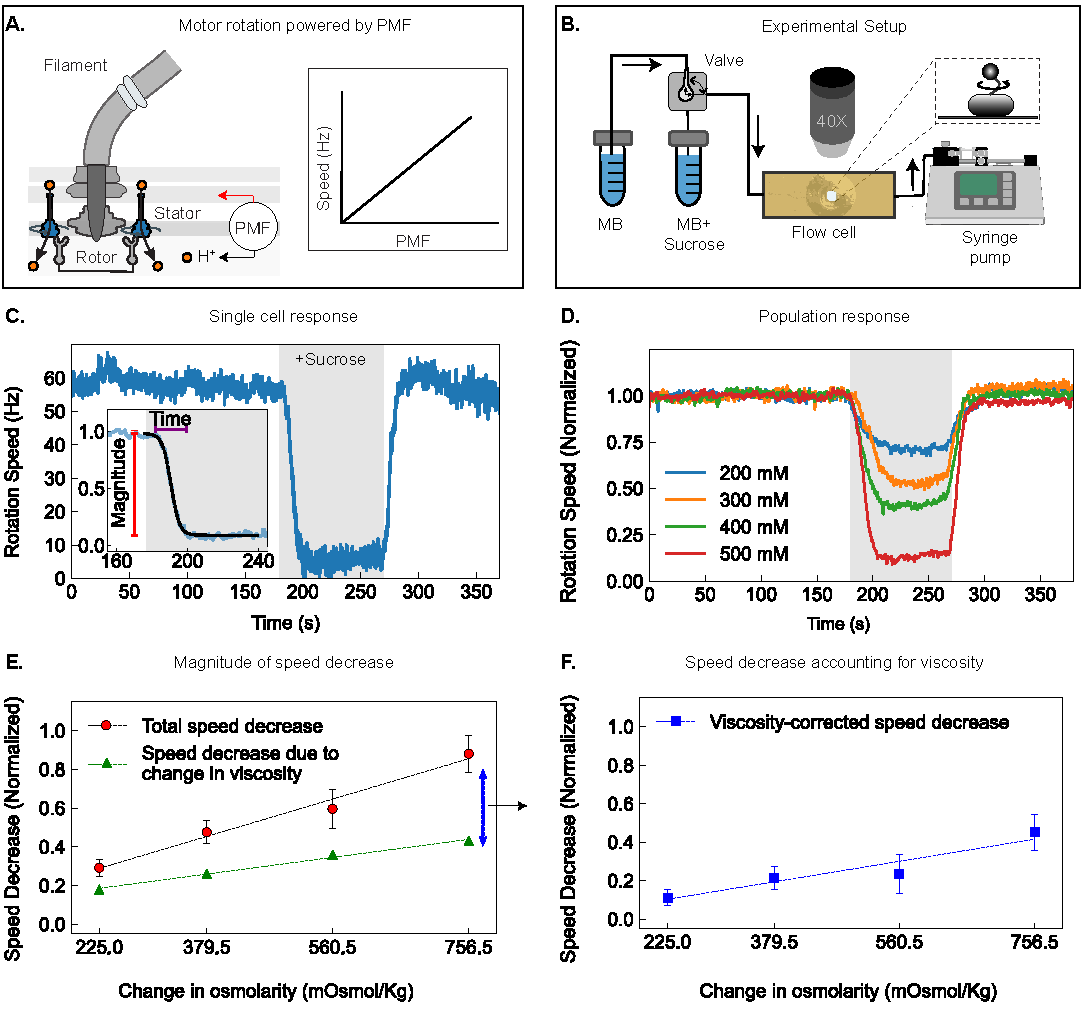
\includegraphics[width=\textwidth]{figures/sucrose.pdf}
    \caption{\textbf{Bacterial flagellar motor response to hyperosmotic shock measured by bead assay.}
    (\textbf{A}) Schematic of the motor, in which proton motive force (PMF) drives rotation via stator units; motor speed is linearly proportional to PMF (inset). (\textbf{B}) Bead assay: A fluidics system alternates between motility buffer (MB) and MB + sucrose. A 1~µm bead attached to the \textit{E. coli} filament tracks motor rotation, imaged with a 40X phase contrast microscope and a high-speed CMOS camera.
    (\textbf{C}) Example trace showing motor speed drop during hyperosmotic shock (gray) and recovery upon removal. At 180~s, media is switched from MB to MB + 500~mM sucrose, then back to MB after 90~s. Inset: Speed normalized to its pre-shock value, with a sigmoidal fit illustrating the magnitude (red bar) and timescale (purple bar) of the reduction.
    (\textbf{D}) Population-averaged responses to 200--500~mM sucrose shocks. Larger shocks produce greater speed reductions. Rotation speeds were normalized to the mean pre-shock speed $\omega_{\mathrm{0}}$ for each condition, $\omega_{\mathrm{norm}}(t) = \omega(t)/\omega_{\mathrm{0}}$. $n=$ 8, 10, 8, and 12, for 200, 300, 400, and 500~mM, respectively. (\textbf{E}) Normalized speed reduction vs. change in osmolarity. Red circles and black  bars show mean and SD; dashed black line is a linear fit. Green triangles and the dashed green line show the estimated viscosity-driven speed decrease and a linear fit to those data. The blue double arrow indicates viscosity-corrected reduction, shown in (\textbf{F}).
    (\textbf{F}) Viscosity-corrected speed decreases; blue squares and error bars show mean and SD; dashed blue line is a linear fit. Fit  parameters are given in  Tables~\ref{tab:fit_only_viscosity} and \ref{tab:fit_all_conditions}.}
    \label{fig:sucrose_MB_shocks} 
\end{figure*}   

\subsection*{Hyperosmotic shock causes rapid reduction of motor rotation speed}

We used the flagellar motor bead assay to monitor PMF in real time. In this assay, a micron-sized bead is attached to the flagellar filament and its rotation is tracked as a direct readout of motor speed and, consequently, PMF (Fig.~\ref{fig:sucrose_MB_shocks}A). Motor rotation is powered by proton flux across stator units embedded in the inner membrane, and rotation speed depends on PMF~\cite{GABEL2003l,Krasnopeeva2024}. While PMF includes contributions from both the membrane potential ($\Delta\psi$) and the pH gradient ($\Delta$pH), all experiments were performed at an external pH of 7.5, where the $\Delta \text{pH}$ is negligible~\cite{padan1976,slonczewski1981}. Thus, any changes in motor speed reflect changes in membrane potential.

To probe the PMF response to a hyperosmotic shock, we immobilized \textit{E. coli} cells inside a custom-made flow cell~\cite{beg_block} and attached 1~µm polystyrene beads to their flagellar stubs. We used a strain expressing a mutant filament protein (FliC-st) to which beads readily adhere, and which lacks the chemotaxis response regulator CheY, so that motors rotate exclusively counterclockwise. Under a constant flow rate set by a syringe pump, the medium could be switched from isotonic to hyperosmotic using a manual valve (Fig.~\ref{fig:sucrose_MB_shocks}B).

Osmotic shock resulted in a rapid reduction in motor rotation speed. After recording the baseline rotation speed of an individual motor in MB for 180~s, we applied a hyperosmotic shock by switching to MB supplemented with 500~mM sucrose (shaded region, Fig.~\ref{fig:sucrose_MB_shocks}C). Prior to the shock, the motor rotated at a stable speed of approximately 50~Hz. Immediately after the shock, motor speed decreased to approximately 10~Hz and remained approximately constant at this minimum for the duration of the shock. After 90~s, the medium was switched back to MB, and motor speed quickly recovered to its original value.

Across different shock strengths, single  motor speeds varied in magnitude but followed similar dynamics (Fig.~\ref{sfig:all_individual_speeds_sucrose}). We tested the cell’s response to MB supplemented with 200~mM, 300~mM, 400~mM, and 500~mM sucrose (Fig.~\ref{fig:sucrose_MB_shocks}D), corresponding to changes in osmolarity of 225, 379.5, 560.5, and 756.5 mOsmol/Kg, respectively (Table~\ref{tab:combined_osmolarity}). Higher sucrose concentrations caused greater reductions in the population-averaged motor speed (Fig.~\ref{fig:sucrose_MB_shocks}D), with the magnitude of speed decrease increased linearly with osmotic upshift strength (Fig.~\ref{fig:sucrose_MB_shocks}E). 

We ruled out increased viscosity as the sole cause for the observed speed reduction. Higher sucrose concentrations increase medium viscosity (Table \ref{tab:viscosity-sucrose}), which raises the viscous drag on the bead and reduces rotation speed. However, the estimated viscosity-driven speed reduction was insufficient to account for the full magnitude of the observed speed loss (Fig.~\ref{fig:sucrose_MB_shocks}E and Fig.~\ref{sfig:viscosity-sucrose}), indicating that hyperosmotic shock induces an additional biophysical effect on motor speed. The viscosity-corrected speed decrease also increased linearly with the change in osmolarity (Fig. \ref{fig:sucrose_MB_shocks}F). The characteristic timescale of motor speed loss was approximately 3~s across all conditions tested and did not vary significantly with shock strength~(Fig.~\ref{sfig:tau-sucro-increa-decrease}), as did the timescale of speed recovery upon return to isotonic medium. These timescales are comparable to those of cell size changes following hyperosmotic shock~(Fig.~\ref{sfig:cell-area}).

These results differ from an earlier report in which motor speed increased above baseline following osmotic upshock at low shock magnitudes~\cite{rosko-2017}. We did not observe a speed increase at low osmolarities (Fig.~\ref{sfig:100mM-sucrose}), nor did addition of osmoprotectants to the medium significantly affect our results~(Fig.~\ref{sfig:200_short_osmopro}). Possible sources of this discrepancy are discussed later.

\begin{figure}[!b]
    \centering
    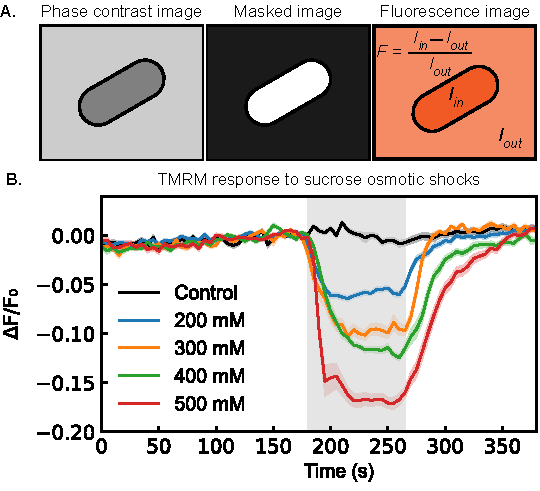
\includegraphics[width=\linewidth]{figures/quantification_TMRM.pdf}
      \caption{\textbf{Hyperosmotic shock induces transient membrane depolarization in \textit{E. coli}.}  \textbf{(A)} Schematic of the analysis pipeline for quantifying the TMRM signal. The cell image was segmented to generate a binary mask defining the intracellular region. The intracellular-to-extracellular fluorescence ratio $F = (I_{\mathrm{in}} - I_{\mathrm{out}})/I_{\mathrm{out}}$ was calculated from the mean fluorescence intensity inside the cell ($I_{\mathrm{in}}$), and the background intensity outside the cell ($I_{\mathrm{out}}$). \textbf{(B)} Population-averaged fluorescence ratios for 200--500~mM sucrose shocks and a 0~mM sucrose control ($n = 40$ per condition), normalized as $\Delta F/F_{0} = (F_{t} - F_{0})/F_{0}$, where $F_{t}$ is the fluorescence ratio at time $t$ and $F_{0}$ is the mean pre-shock value. Upon osmotic shock, fluorescence decreased in a dose-dependent manner and recovered to pre-shock values upon return to base media. Solid lines and shaded bands represent mean and SE.}
    \label{fig:TMRM}
\end{figure}

\subsection*{TMRM labeling reveals membrane depolarization during osmotic shock} 
As noted before, $\Delta$pH is expected to be negligible at an external pH of 7.5~\cite{padan1976,slonczewski1981}. Thus, any changes in PMF must be due to changes in membrane potential. To test whether the motor response to osmotic shock is associated with depolarization, we performed the sucrose shock experiments again, this time using \textit{E. coli} cells labeled with the Nernstian dye Tetramethylrhodamine methyl ester (TMRM) and using its fluorescence intensity as a proxy for dye concentration~\cite{LO2007etl,KRASNOPEEVA2019l}. TMRM molecules distribute across the membrane according to the Nernst equation, $\Delta\psi = -\frac{RT}{zF} \ln (\frac{c_{in}} {c_{out}})$, where $\Delta\psi$ is the membrane potential and $\frac{c_{in}} {c_{out}}$ is the ratio of intracellular to extracellular TMRM concentration at equilibrium~\cite{Ehrenberg1988membrane,Farkas1989simultaneous,BENARROCH2020304l}. A decrease in membrane potential reduces intracellular dye accumulation and, consequently, the fluorescence signal~\cite{jinetal2023l,KRASNOPEEVA2019l}. We quantified the intracellular-to-extracellular TMRM fluorescence ratio by measuring the mean intracellular intensity relative to the local background, expressed as $(I_{\mathrm{in}} - I_{\mathrm{out}})/I_{\mathrm{out}}$, using a cell segmentation mask derived from phase contrast images (Fig.~\ref{fig:TMRM}A). This value was further normalized to the pre-shock baseline and reported as $\Delta F/F_{0}$ (see Methods).

The intracellular-to-extracellular TMRM fluorescence ratio decreased rapidly after osmotic shock, indicating membrane depolarization and, consequently, a reduction in PMF (Fig.~\ref{fig:TMRM}B). As with motor speed, the magnitude of the decrease in TMRM signal increased with shock strength, while the timescale of the response showed no consistent trend. However, the timescales of TMRM signal decrease and recovery were more variable than those of motor speed, ranging between 2.7~s and 15.7~s~(Fig. \ref{sfig:timescale-TMRM}). This is expected, as these timescales reflect both the dynamics of PMF change and the exchange of TMRM between the cell and the surrounding medium. Nevertheless, the clear shock-dependent change in TMRM signal following osmotic shock is consistent with disruption of the membrane potential.


\begin{figure}[!t]
    \centering
    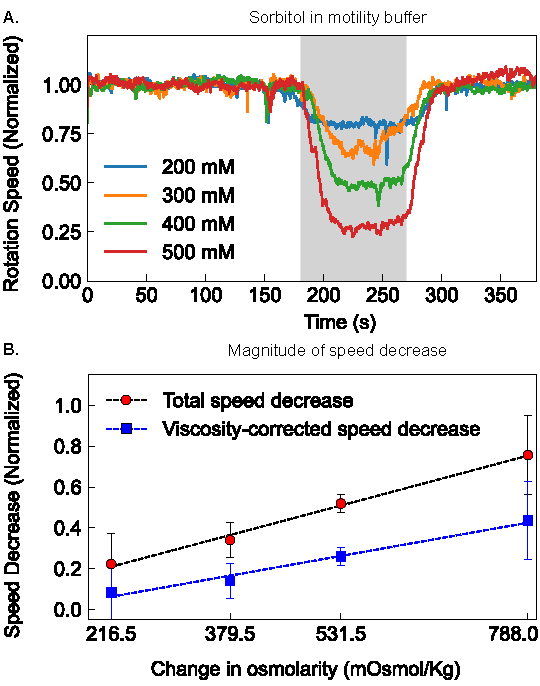
\includegraphics[width=\linewidth]{figures/sorbitol-biophysics.pdf}
    \caption{\textbf{Motor response to osmotic shock is independent of the choice of non-ionic osmolyte.}
    (\textbf{A}) Population-averaged normalized rotation speed during 200--500~mM sorbitol shocks ($n= 8$ per condition). Rotation speeds were normalized to the mean pre-shock speed $\omega_{\mathrm{0}}$ for each condition, $\omega_{\mathrm{norm}}(t) = \omega(t)/\omega_{\mathrm{0}}$. The shaded region indicates the duration of hyperosmotic exposure. 
    (\textbf{B}) Normalized speed reduction vs.\ change in osmolarity for sorbitol shocks. Red circles and black error bars represent the mean and SD of the total normalized speed decrease; the dashed black line is a linear fit. Blue squares and error bars show the viscosity-corrected speed decrease, with the dashed blue line representing a linear fit to the corrected values. Fit parameters are provided in Table \ref{tab:fit_all_conditions}.}
    \label{fig:sorb_MB_shocks}
\end{figure}

\vspace{-1em} % optional small adjustment
\noindent

\subsection*{Response to osmotic shock is independent of the choice of non-ionic osmolyte}

Next, we tested whether the observed response depended on the choice of non-ionic osmolyte. We avoided ionic osmolytes such as NaCl, as they can alter the membrane potential independently of osmolarity~\cite{berscheid2024}. As an alternative, we chose sorbitol, which, like sucrose, is uncharged and non-metabolized, and enters the periplasm rapidly but is taken up into the cytoplasm slowly~\cite{stephens2024scr,rojas2014}. Population-averaged motor speed traces for 200--500~mM sorbitol shocks closely resembled those obtained with sucrose (Fig.~\ref{fig:sorb_MB_shocks}A): motor speed dropped sharply upon upshift, stabilized at a minimum, and recovered quickly upon return to isotonic MB. The characteristic timescale of speed loss was largely independent of sorbitol concentration and remained on the order of 5~s (Fig.~\ref{sfig:tau-sorb-sodium-clock}A). 

As with sucrose, increasing sorbitol concentration raised medium viscosity (Table \ref{tab:viscosity-sorb}), but the viscosity-driven speed reduction again did not fully account for the observed speed loss (Fig.~\ref{fig:sorb_MB_shocks}B and Fig.~\ref{sfig:viscosity-plot-Sorb}). Furthermore, although the total speed decrease was smaller with sorbitol than with sucrose due to its lower effect on viscosity, the viscosity-corrected speed loss was identical for the two osmolytes (Fig.~\ref{sfig:tau-sorb-sucrose-combine}). Together, these results indicate that the viscosity-corrected speed loss reflects a common cellular response to osmotic stress, consistent with PMF disruption, rather than a specific effect of either solute.

\begin{figure}[!b]
    \centering
    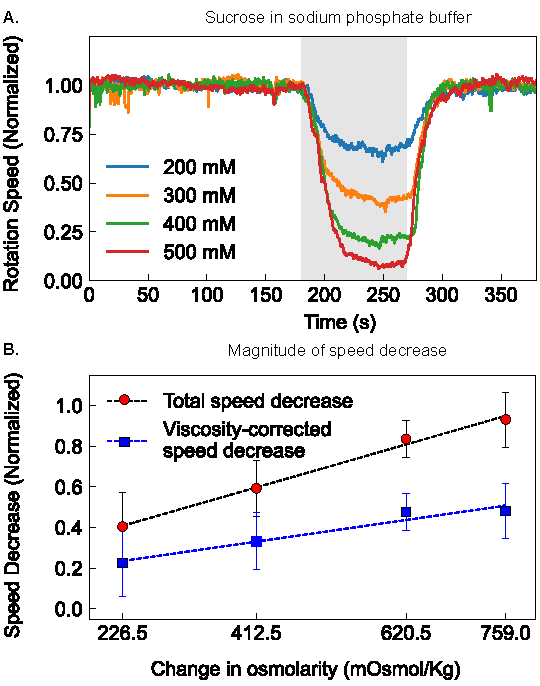
\includegraphics[width=\linewidth]{figures/sodium-biophysics.pdf}
    \caption{\textbf{Motor response to osmotic shock is independent of buffer composition.} (\textbf{A}) Population-averaged normalized rotation speed during 200--500~mM sucrose shocks in sodium phosphate buffer (SPB) ($n = 10$ per condition). Rotation speeds were normalized to the mean pre-shock speed $\omega_{\mathrm{0}}$ for each condition, $\omega_{\mathrm{norm}}(t) = \omega(t)/\omega_{\mathrm{0}}$. The shaded region indicates the duration of hyperosmotic exposure. (\textbf{B}) Normalized speed reduction vs.\ change in osmolarity for SPB shocks. Red circles and black error bars represent the mean and SD of the total normalized speed decrease; the dashed black line is a linear fit. Blue squares and error bars show the viscosity-corrected speed decrease, with the dashed blue line representing a linear fit to the corrected values. Fit parameters are provided in Table~\ref{tab:fit_all_conditions}.}
    \label{fig:sodium}
\end{figure}


\subsection*{Rotation speed decrease does not require potassium ions}

Potassium uptake is a key component of \textit{E. coli}'s response to hyperosmotic shock~\cite{STAUTZ20211,dinnbier1988transientl}, and a rapid influx of positively charged ions could in principle influence membrane potential. To test whether potassium uptake contributes to the observed motor response, we repeated the sucrose shock experiments using sodium phosphate buffer (SPB) as the base medium in place of MB, removing potassium from the system entirely. The motor response in SPB closely resembled that in MB across all shock strengths (Fig.~\ref{fig:sodium}A): the magnitude of speed loss scaled with osmolarity, the viscosity correction did not fully account for the observed decrease (Fig.~\ref{fig:sodium}B), and the timescale of speed loss was independent of shock strength (Fig.~\ref{sfig:tau-sorb-sodium-clock}B). Thus, while potassium uptake contributes to long-term osmotic adaptation~\cite{dinnbier1988transientl}, it is not required for the immediate PMF response to hyperosmotic shock.

 \begin{figure}[!t]
    \centering
    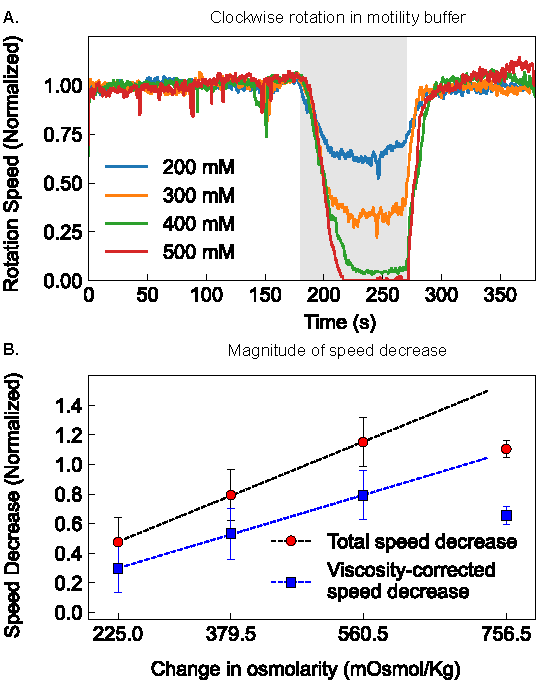
\includegraphics[width=\linewidth]{figures/clockwise-biophyscis.pdf}
    \caption{\textbf{Motor speed reduction is independent of the direction of rotation.}
    (\textbf{A}) Population-averaged normalized rotation speed during 200--500~mM sucrose shocks in \textit{E. coli} cells locked in clockwise (CW) rotation ($n = 8$ per condition). Rotation speeds were normalized to the mean pre-shock speed $\omega_{\mathrm{0}}$ for each condition, $\omega_{\mathrm{norm}}(t) = \omega(t)/\omega_{\mathrm{0}}$. The shaded region indicates the duration of hyperosmotic exposure.
    (\textbf{B}) Normalized speed reduction vs.\ change in osmolarity for CW motors. Red circles and black error bars represent the mean and SD of the total normalized speed decrease; the dashed black line is a linear fit. Blue squares and error bars show the viscosity-corrected speed decrease, with the dashed blue line representing a linear fit to the corrected values. Because motor speed reached 0~Hz at 500~mM sucrose, saturating the response, only 200--400~mM conditions were used to compute the fits. Fit parameters are provided in Table~\ref{tab:fit_all_conditions}.}
    \label{fig:clockwise}
\end{figure}

% \vspace{-1em} % optional small adjustment
% \noindent


\subsection*{Motor speed response is independent of rotor conformation}

The bacterial flagellar motor can rotate in either the counterclockwise (CCW) or clockwise (CW) direction, and the two configurations involve dramatically different conformational states of the C-ring rotor~\cite{chang2020,johnson2024,singh2024}. If the observed speed reduction were due to a specific perturbation of the stator-rotor interface --- for instance, osmotic stress disrupting rotor conformation or stator-rotor binding --- one might expect the response to differ between CCW and CW motors. To test this, we repeated the sucrose shock experiments using a strain that overexpresses CheY from an IPTG-inducible plasmid, locking motors in exclusive CW rotation.

The response of CW motors to hyperosmotic shock closely followed that of CCW rotating motors (Fig.~\ref{fig:clockwise}A). Speed dropped sharply upon upshift, the viscosity correction did not account for the full speed loss (Fig.~\ref{fig:clockwise}B), and the timescale of speed decrease was independent of shock strength (Fig.~\ref{sfig:tau-sorb-sodium-clock}C). The similarity of the response across two structurally distinct rotor configurations indicates that the effect does not originate at or downstream of the stator-rotor interface. Instead, it points to a perturbation that acts upstream, most likely at the level of the proton motive force that energizes the stator, consistent with our interpretation of PMF disruption.

 \begin{figure}[!b]
    \centering
    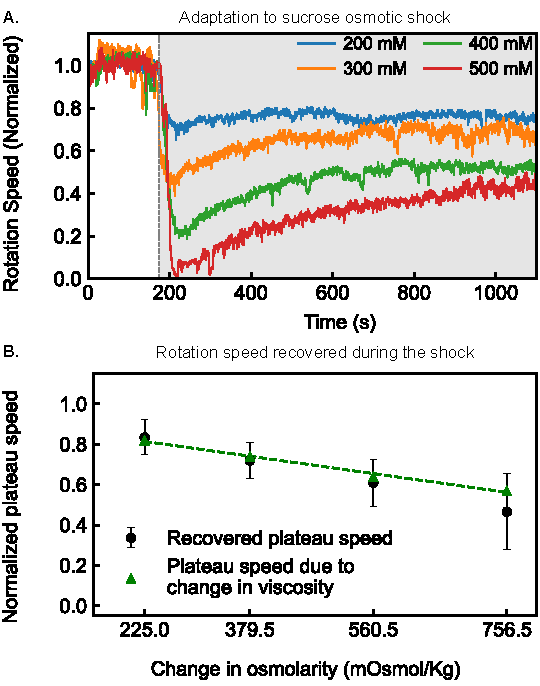
\includegraphics[width=\linewidth]{figures/osmoadaption-biophysics.pdf}
    \caption{\textbf{Adaptation of flagellar motor speed following hyperosmotic shock.} 
    \textbf{(A)} Time courses of normalized flagellar motor rotation speed after application of sucrose osmotic shocks of different magnitudes (200--500 mM). The dashed vertical line indicates the time at which the hyperosmotic medium was introduced. Motor speed drops rapidly following the shock and then partially recovers over several minutes to a new steady plateau whose level depends on the shock strength. Traces represent the mean of $n = 8, 8, 8,$ and $4$ motors for 200~mM, 300~mM, 400~mM, and 500~mM sucrose upshifts, respectively, normalized to the pre-shock speed.
    \textbf{(B)} Plateau motor speed measured several minutes after the shock as a function of the change in osmolarity. Black circles and black error bars represent the mean and SD, respectively. Green triangles indicate the plateau speed expected from the increase in medium viscosity due to sucrose alone.}
    \label{fig:osmoadaption}
\end{figure}

% \vspace{-1em} % optional small adjustment
% \noindent

\subsection*{Adaptation of motor rotation speed during sustained osmotic shock} To examine the longer-term PMF response to osmotic stress, we monitored motor rotation speed under sustained hyperosmotic shock, allowing sufficient time for cellular adaptation mechanisms to engage~\cite{dinnbier1988transientl,bremer2019responses,wood2010,wood2011bacterial,wood2015}. Upon application of the hyperosmotic medium, motor speed decreased rapidly and then gradually recovered over several minutes to a new steady plateau (Fig.~\ref{fig:osmoadaption}A), in agreement with earlier work~\cite{rosko-2017}. The magnitude of the initial decrease increased with shock strength, and despite partial recovery, the final plateau speed remained below the pre-shock value and decreased systematically with increasing osmolarity.

To quantify this behavior, we measured the steady plateau speed reached several minutes after the shock and compared it to the speed reduction expected from the increase in medium viscosity alone. Within experimental uncertainty, the measured plateau speeds were consistent with the viscosity-based predictions (Fig.~\ref{fig:osmoadaption}B). This agreement indicates that, following adaptation, PMF recovers to approximately its pre-shock value, and the remaining reduction in motor speed is largely accounted for by the increased viscous load imposed by the sucrose solution.

\section*{Discussion}

Osmotic stress is widely studied as a mechanical and chemical challenge to bacterial cells, but its impact on cellular energetics has received comparatively little attention. Our results demonstrate that hyperosmotic shock rapidly depolarizes \textit{E. coli}, revealing PMF disruption as an underappreciated component of the osmotic stress response. The effect is dose-dependent, reversible, and reproducible across different osmolytes, buffer compositions, and motor configurations, pointing to a general cellular response rather than an artifact of experimental conditions. The convergence of two independent measurements---flagellar motor speed and TMRM fluorescence---on the same conclusion strengthens this interpretation considerably.

We used the bacterial flagellar motor as a real-time reporter to monitor PMF with high temporal resolution. Unlike fluorescence-based methods, which require exogenous dyes that can themselves perturb PMF~\cite{MANCINI20204l}, motor rotation is intrinsic to the cell's biology and can be measured noninvasively from outside the cell. Because PMF is spatially homogeneous within the cell~\cite{biquet2024spatiotemporal}, the speed of a single motor reflects the global energetic state of the cell. Although the precise quantitative dependence of motor speed on PMF has been debated~\cite{fung_berg1995,GABEL2003l,Krasnopeeva2024}, the relationship is consistently monotonic,  making motor speed a reliable proxy for relative changes in PMF.

Our TMRM measurements provide independent support for the motor’s reliability as a reporter of PMF. At the external pH of $\sim$7.5 used in our experiments, $\Delta \text{pH}$ is negligible and the membrane potential therefore constitutes the dominant component of the PMF~\cite{padan1976,slonczewski1981}. To minimize dye-induced perturbation of membrane potential, we used low TMRM concentrations that have been reported to reduce quenching, aggregation, and membrane disruption~\cite{LO2007etl,jinetal2023l}. Under these conditions, the intracellular-to-extracellular fluorescence ratio decreased in a shock-dependent manner, mirroring the changes in motor speed. While TMRM fluorescence intensity does not necessarily scale linearly with dye concentration and therefore does not permit precise membrane potential estimates via the Nernst equation, it nevertheless provides a qualitative indicator of PMF dynamics across different osmotic shock strengths. Thus, while motor measurements report on flagellar rotation and TMRM assays report on dye distribution across the membrane, both independently indicate that hyperosmotic shock depolarizes \textit{E. coli}.

While our measurements consistently reveal a clear PMF decrease following hyperosmotic shock, our findings differ in an important respect from those of Rosko et al.~\cite{rosko-2017}, who reported an \textit{increase} in motor speed above baseline following osmotic upshock, with a transient speed drop observed at higher shock strengths. In contrast, we consistently observed a \textit{decrease} in motor speed, which we interpret as a reduction in PMF. Several methodological differences, including bead size, osmotic media delivery method, and flow cell geometry, may contribute to this discrepancy.  The absence of any effect from the addition of osmoprotectants to our media argues against buffer composition as an explanation for the divergent results. Reconciling these differences represents an important open question for future work.

As an external stimulus, hyperosmotic stress reduces turgor pressure and alters cell shape and volume~\cite{pilizota_2012,pilizota2013plasmolysis,Rojas2020}. These changes activate osmoresponsive channels that help restore turgor pressure and cell shape~\cite{sleator_hill}. Our data suggest that, beyond these mechanical and structural effects, hyperosmotic stress may also perturb cellular energetics by inducing a loss of PMF. Conversely, hypo-osmotic shock activates mechanosensitive (MS) channels that mediate rapid ion efflux~\cite{wood2010,bremer2019responses}. Because ion flux directly contributes to the electrochemical gradient across the membrane, activation of these channels could also alter the cellular PMF, an effect that would be detectable with our assays. Although our study focused primarily on hyperosmotic stress, extending these measurements to hypo-osmotic conditions could provide further insight into how osmotic perturbations impact bacterial energetics.

Osmotic stress triggers rapid physical and chemical changes within seconds~\cite{pilizota_2012}, and our motor experiments provide the temporal resolution needed to capture the PMF response in this initial window. The characteristic timescale of motor speed decrease is a few seconds (Fig.~\ref{sfig:tau-sucro-increa-decrease}), and because the estimated media exchange time is much shorter ($\sim400~\textrm{ms}$; see Supporting Information), this reflects the intrinsic cellular response rather than the kinetics of the delivery of osmotic shock.

On longer timescales, our sustained shock experiments reveals that PMF recovers over several minutes --- dynamics that were likely missed in earlier studies reporting no significant changes in PMF several minutes after shock~\cite{HOUSSIN1991,shabala_2009}. This recovery timescale is consistent with that of cellular volume recovery following osmotic shock~\cite{pilizota_2012,rosko-2017}, suggesting that the two processes are coupled. Since protein synthesis occurs on longer timescales than those we observe~\cite{poolman2002membrane,weber2006time}, PMF recovery is most likely mediated by pre-existing adaptation mechanisms~\cite{sleator_hill,wood2010,poolman2023} rather than new protein production.

The rapid timescale of motor speed change in our experiments argues against stator remodeling as the primary mechanism. PMF is known to regulate stator engagement with the motor~\cite{fung_berg1995,tipping2013quantification}. However, both the decrease upon shock ($\sim 3\,\mathrm{s}$) and the recovery upon its removal ($\sim 3\,\mathrm{s}$) are far faster than reported timescales for stator disassembly and assembly, which range from $\sim10$ to $500\,\mathrm{s}$ under PMF-dependent or load-dependent remodeling conditions~\cite{tipping2013quantification,lele2013,nord2017catch,wadhwaphillipsberg2019,wadhwa2021}. For reference, sodium azide-induced stator disassembly occurs on a timescale of $\sim26\,\mathrm{s}$~\cite{tipping2013quantification}, and stator assembly following load-dependent remodeling in the strain used here occurs on a timescale of $\sim50\,\mathrm{s}$~\cite{wadhwaphillipsberg2019,wadhwa2021}, which are both at least an order of magnitude slower than the response we observe. Together, these comparisons suggest that stators likely remain bound throughout the osmotic shocks. However, since stator dynamics were not directly monitored in our experiments, remodeling cannot be formally ruled out. Whether the depolarization we observe leads to any stator rearrangement on longer timescales remains an open question.

While the precise molecular mechanism by which hyperosmotic shock disrupts membrane potential remains unclear, osmotic stress is known to broadly perturb cellular metabolism and respiration~\cite{roth1985osmotic,HOUSSIN1991,meury1994immediate}. Rapid inhibition of carbon uptake~\cite{roth1985osmotic} and decreases in respiratory activity~\cite{meury1994immediate,HOUSSIN1991} under osmotic stress suggest that proton-pumping processes may be transiently compromised. Hyperosmotic stress causes rapid water efflux through AqpZ~\cite{poolman2002membrane,wood2010,wood2015}, leading to cell shrinkage, changes in membrane tension~\cite{sleator_hill,sun2021}, and alterations in the cytoplasmic physicochemical state, including ionic strength, pH, and macromolecular crowding~\cite{chakraborty2017non,liu2019decreased,sikkema2020gating,poolman2023}. Changes in membrane tension could directly perturb the conformation and proton-pumping activity of ETC complexes embedded in the inner membrane; Complex I, for instance, undergoes conformational transitions linked to its catalytic state~\cite{agip2018}, and its activity may be sensitive to the lipid environment of the inner membrane~\cite{gutierrez2020key,phillips2009}. Together these biophysical and metabolic perturbations could impair proton pumping and reduce membrane potential. The rapid timescale of motor slowdown observed here argues against transcriptional or translational responses, pointing instead toward an immediate biophysical or metabolic mechanism~\cite{poolman2002membrane,weber2006time}. Mechanical perturbations have previously been shown to induce calcium influx and membrane depolarization in bacteria~\cite{bruni2017}; however,
this mechanism is unlikely to explain our observations, as our experimental media contained no calcium. Elucidating the mechanism linking osmotic stress to PMF disruption remains an important open question for future work.

\section*{Acknowledgments}
We thank Daozheng Gong for preliminary data collection, Shabduli Sawant and Brennen Wise for their assistance with data analysis, and members of the Wadhwa Lab for helpful discussions. We are grateful to Drs. Jeremy Wideman and David Blair for feedback on the manuscript.

\section*{Funding}
 N.W. is supported by the National Institute of General Medical Sciences of the National Institutes of Health grant R00GM134124 and by the Arizona Biomedical Research Centre grant RFGA2023-008-14.
 
\section*{Author contributions}
N.W. designed research; L.M., S.B., and J.Y. performed research; L.M., F.J., and E.D. analyzed data; L.M., F.J., and N.W. wrote the paper. 

\section*{Competing interests}
The authors declare no competing interests.

\section*{Data and materials availability}
All code and data used in this manuscript are available at the GitHub repository: \url{https://github.com/wadhwalab/hyperosmotic.git}.

\section*{SUPPORTING CITATIONS}
References \cite{swindells1958,Sahare2021} appear in the Supporting Material.

\section*{SUPPORTING MATERIAL}
An online supplement to this article can be found by visiting BJ 
Online at \url{http://www.biophysj.org}.

% Uncomment if using bibtex (default)
\bibliography{REFERENCES}

\end{document}
